\section{Pruebas técnicas y resultados}\label{sec:resultados}

Todas las cifras de esta sección salen de los archivos de la carpeta \texttt{results/} y se regeneran con el script \texttt{make\_tables.py} de la carpeta \texttt{bench/}. Todas las cubiertas óptimas que reporta cualquiera de nuestros algoritmos exactos coinciden entre sí y con los valores publicados por \textsc{WeGotYouCovered}. No encontramos ninguna discrepancia.

\subsection{Algoritmos exactos}
La \cref{tab:exactos} cuenta cuántas instancias resuelve cada algoritmo exacto con optimalidad probada en 10\,s, y la \cref{fig:cactus} muestra el número de instancias resueltas del PACE~2019 en función del tiempo.

\begin{table}[!htbp]\centering\small
\begin{tabular}{@{}lrrrrrrrr@{}}\toprule
 & \multicolumn{2}{c}{\alg{PD-TD}} & \multicolumn{2}{c}{\alg{DyV-WH}} & \multicolumn{2}{c}{\hyvc} & \multicolumn{2}{c}{\textsc{WeGotYouCovered}$^\dagger$} \\\cmidrule(lr){2-3}\cmidrule(lr){4-5}\cmidrule(lr){6-7}\cmidrule(l){8-9}
Conjunto & res. & $\tilde t$ (s) & res. & $\tilde t$ (s) & res. & $\tilde t$ (s) & res. & $\tilde t$ (s) \\\midrule
PACE 2019 (200) & 13 & 0.29 & 13 & 0.01 & 30 & 0.00 & 155 & 2.10 \\
PACE 2017 (200) & 137 & 0.00 & 65 & 0.12 & 198 & 0.00 & \multicolumn{2}{c}{---} \\
Sintéticas (35) & 8 & 0.01 & 5 & 0.00 & 25 & 0.00 & \multicolumn{2}{c}{---} \\
\bottomrule\end{tabular}
\caption{Instancias resueltas con optimalidad probada en 10\,s y mediana del tiempo sobre las resueltas. $^\dagger$Tiempos publicados por sus autores~\citep{hespe2020} en su propio hardware; se cuentan las instancias que resolvió en 10\,s o menos.}\label{tab:exactos}\end{table}


\begin{figure}[!htbp]
\centering
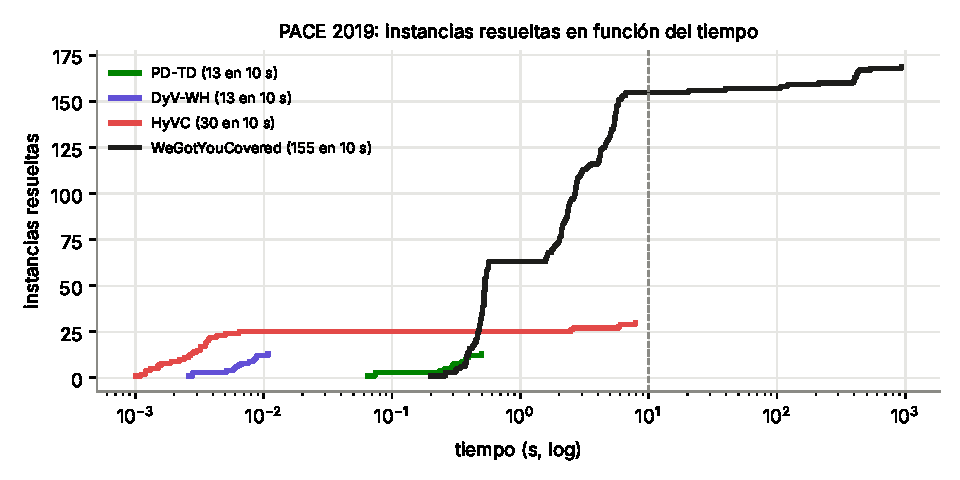
\includegraphics[width=0.88\textwidth]{figs/pace2019_cactus.pdf}
\caption{PACE 2019: instancias resueltas en función del tiempo. Nuestros algoritmos tienen un límite de 10\,s (línea punteada). Los tiempos de \textsc{WeGotYouCovered} son los publicados por sus autores~\citep{hespe2020}, con un límite de 30 minutos en su propio hardware.}
\label{fig:cactus}
\end{figure}

\paragraph{Frente a los algoritmos base.} \hyvc{} resuelve más instancias que la PD y que el divide y vencerás en los tres conjuntos: 30 frente a 13 y 13 en el PACE~2019, 198 frente a 137 y 65 en el PACE~2017, y 25 frente a 8 y 5 en las sintéticas. Además, toda instancia resuelta por la PD o por el divide y vencerás también la resuelve \hyvc{} (\cref{tab:sinteticas}). El divide y vencerás sin cotas solo termina cuando el grafo se fragmenta rápido. En 8 instancias grandes del PACE~2019 lo mató el sistema por falta de memoria: cada nivel de la recursión copia el grafo residual. La PD resuelve exactamente las 137 instancias del PACE~2017 cuyo ancho de eliminación es $\le 22$, y ninguna otra.

\paragraph{Frente al estado del arte.} En el PACE~2019, \textsc{WeGotYouCovered} resuelve 155 instancias en 10\,s o menos, y 169 en el límite oficial de 30 minutos~\citep{hespe2020}. Las 30 que resuelve \hyvc{} están todas entre esas 155, así que \hyvc{} no resuelve ninguna que el ganador no resuelva. La diferencia es grande y la explicamos en la \cref{sec:fallos}. En las 30 que sí resuelve, \hyvc{} es más rápido (mediana de 3\,ms frente a 0.53\,s), pero son las instancias fáciles: 25 de ellas se resuelven solo con las reglas de reducción.

\subsection{Calidad de las heurísticas}
La \cref{tab:calidad} compara las cubiertas con el óptimo en las instancias donde está certificado.

\begin{table}[!htbp]\centering\small\setlength{\tabcolsep}{4pt}
\begin{tabular}{@{}lrrrrrrrr@{}}\toprule
 & \multicolumn{2}{c}{\alg{Voraz-WH}} & \multicolumn{2}{c}{MIS ($R{=}1$)} & \multicolumn{2}{c}{MIS ($R{=}64$)} & \multicolumn{2}{c}{\hyvc} \\\cmidrule(lr){2-3}\cmidrule(lr){4-5}\cmidrule(lr){6-7}\cmidrule(l){8-9}
Conjunto (con óptimo) & $\overline{|C|/\tau}$ & $=\tau$ & $\overline{|C|/\tau}$ & $=\tau$ & $\overline{|C|/\tau}$ & $=\tau$ & $\overline{|C|/\tau}$ & $=\tau$ \\\midrule
PACE 2019 (96) & 1.027 & 14 & 1.066 & 13 & 1.047 & 13 & 1.013 & 30 \\
PACE 2017 (198) & 1.031 & 44 & 1.099 & 8 & 1.049 & 28 & 1.000 & 198 \\
Sintéticas (25) & 1.412 & 0 & 1.264 & 1 & 1.110 & 4 & 1.000 & 25 \\
\bottomrule\end{tabular}
\caption{Calidad de las cubiertas en las instancias con óptimo certificado: razón media $|C|/\tau$ y número de instancias donde el algoritmo encontró el óptimo.}\label{tab:calidad}\end{table}


\begin{itemize}
  \item \textbf{El voraz es la mejor heurística en grafos ``naturales''.} En el PACE~2019 y el PACE~2017 queda en promedio entre un 2.7\,\% y un 3.1\,\% por encima del óptimo, y encuentra el óptimo en 14 y 44 instancias respectivamente.
  \item \textbf{El MIS aleatorio es peor en promedio, pero inmune a la trampa.} Una sola corrida queda entre un 6.6\,\% y un 9.9\,\% por encima del óptimo; con $R=64$ corridas (Monte Carlo) la distancia baja a cerca del 5\,\%. En la trampa de Johnson ocurre lo contrario: el voraz alcanza una razón de 682 vértices frente a $k=160$, una razón de 4.26, mientras el MIS aleatorio encuentra el óptimo en las cuatro instancias. La media de 1.412 del voraz en las sintéticas se debe casi por completo a esa familia. Es exactamente lo que predicen el análisis de Johnson~\citep{johnson1974} y la garantía de Veldt~\citep{veldt2024}.
  \item \textbf{La respuesta \emph{anytime} de \hyvc{}.} En las 170 instancias del PACE~2019 que no resuelve en 10\,s, su cubierta queda en promedio un 0.74\,\% por encima del óptimo o de la mejor conocida, con un máximo de 6.6\,\%.
\end{itemize}

\subsection{Tipos de grafos}
La \cref{tab:sinteticas} separa los resultados por familia sintética.

\begin{table}[!htbp]\centering\small
\begin{tabular}{@{}lrrrrrrr@{}}\toprule
 & \multicolumn{2}{c}{$|C|/\tau$} & \multicolumn{3}{c}{exactas en 10\,s} & & \\\cmidrule(lr){2-3}\cmidrule(lr){4-6}
Familia & Voraz & MIS ($R{=}64$) & PD & DyV & \hyvc & $\tilde t_{\hyvc}$ (s) & núcleo \\\midrule
ER $c{=}1$ & 1.019 & 1.094 & 3/3 & 3/3 & 3/3 & 0.00 & 0\,\% \\
ER $c{=}2$ & 1.044 & 1.117 & 0/3 & 0/3 & 3/3 & 0.00 & 0\,\% \\
ER $c{=}3$ & 1.058 & 1.122 & 0/3 & 0/3 & 3/3 & 0.00 & 4\,\% \\
ER $c{=}4$ & 1.061 & 1.117 & 0/3 & 0/3 & 0/3 & --- & 52\,\%$^{*}$ \\
ER $c{=}6$ & 1.058 & 1.107 & 0/3 & 0/3 & 0/3 & --- & 89\,\%$^{*}$ \\
BA $m{=}2$ & 1.017 & 1.151 & 0/2 & 0/2 & 2/2 & 0.00 & 0\,\% \\
BA $m{=}3$ & 1.027 & 1.138 & 0/2 & 0/2 & 2/2 & 0.00 & 0\,\% \\
BA $m{=}5$ & 1.039 & 1.131 & 0/2 & 0/2 & 0/2 & --- & 100\,\%$^{*}$ \\
Banda $b{=}8$ & 1.043 & 1.089 & 2/2 & 0/2 & 2/2 & 0.00 & 5\,\% \\
Banda $b{=}12$ & 1.036 & 1.075 & 2/2 & 0/2 & 2/2 & 0.13 & 96\,\% \\
Banda $b{=}16$ & 1.035 & 1.064 & 0/2 & 0/2 & 0/2 & --- & 99\,\%$^{*}$ \\
Bipartito $c{=}3$ & 1.063 & 1.127 & 0/2 & 0/2 & 2/2 & 0.00 & 0\,\% \\
Bipartito $c{=}6$ & 1.227 & 1.296 & 0/2 & 0/2 & 2/2 & 0.00 & 41\,\% \\
Trampa & 3.278 & 1.000 & 1/4 & 2/4 & 4/4 & 0.00 & 0\,\% \\
\bottomrule\end{tabular}
\caption{Instancias sintéticas por familia. ``Núcleo'' es la fracción de vértices que sobrevive a las reducciones de \hyvc. $^{*}$Familia con alguna instancia sin óptimo certificado: la razón se calcula contra la mejor cubierta conocida.}\label{tab:sinteticas}\end{table}


\begin{itemize}
  \item \textbf{Erdős--Rényi.} Con $c\le 3$, las reducciones dejan un núcleo de a lo sumo el 4\,\% de los vértices y \hyvc{} resuelve todo al instante; la PD y el divide y vencerás solo resuelven $c=1$. Con $c\ge 4$ el núcleo retiene entre el 52\,\% y el 89\,\% de los vértices y ningún algoritmo termina en 10\,s, ni siquiera CP-SAT en 30\,s. El salto ocurre entre $c=3$ y $c=4$, alrededor del umbral $c=e\approx 2.72$ de Weigt y Hartmann~\citep{weigt2000}.
  \item \textbf{Barabási--Albert.} Con $m\le 3$ las reducciones lo resuelven todo; con $m=5$ no reducen nada y nadie termina.
  \item \textbf{Bandas.} Es el régimen de la PD. Con $b=8$ el ancho de eliminación es 11 y las reducciones ya bastan. Con $b=12$ el ancho es 18--19: la PD resuelve en una décima de segundo, y \hyvc{} la despacha y también. Con $b=16$ el ancho es 26--27 y ningún algoritmo termina.
  \item \textbf{Bipartitos.} Con $c=3$ las reglas los reducen por completo; con $c=6$ queda un 41\,\% de los vértices, pero la cota LP, exacta en bipartitos, cierra la búsqueda de inmediato. \hyvc{} los resuelve todos al instante, mientras el voraz llega a un 22.7\,\% por encima del óptimo con $c=6$.
\end{itemize}

\paragraph{Ancho de árbol real frente a heurístico.} La \cref{fig:anchos} compara, en el PACE~2017, el ancho de la descomposición por grado mínimo con el ancho de árbol exacto. La mediana es de 16 frente a un ancho exacto mediano de 11: en promedio la heurística sobreestima el ancho un 31\,\% y lo acierta en 22 de 200 instancias. Hay 148 instancias con ancho exacto $\le 20$, pero solo 137 con ancho heurístico $\le 22$. La calidad de la descomposición decide entonces en qué instancias se puede usar la PD, como señalan Bannach y Berndt~\citep{bannach2019}.

\begin{figure}[!htbp]
\centering
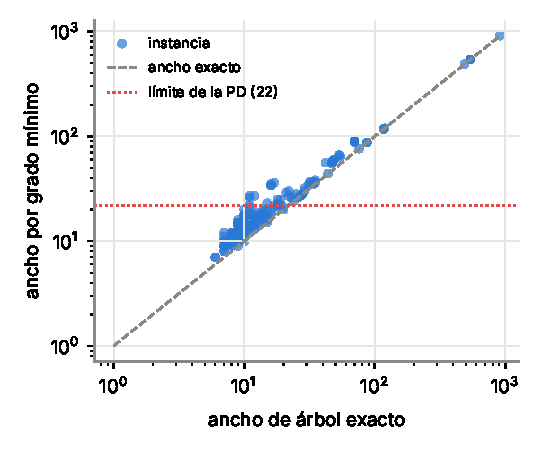
\includegraphics[width=0.5\textwidth]{figs/pace2017_width.pdf}
\caption{PACE 2017: ancho de la eliminación por grado mínimo frente al ancho de árbol exacto, ambos en escala logarítmica. La línea roja es el ancho máximo que acepta nuestra PD.}
\label{fig:anchos}
\end{figure}

\subsection{Qué fase hace el trabajo: ablación}
La \cref{tab:ablacion} apaga una fase de \hyvc{} a la vez.

\begin{table}[!htbp]\centering\small
\begin{tabular}{@{}llrrr@{}}\toprule
Familia & Variante & $\bar t$ (s) & exactas & nodos \\\midrule
Erdős–Rényi $n{=}200$ & HyVC completo & 0.37 & 10/10 & 481 \\
 & sin reducciones & 5.38 & 6/10 & 44 \\
 & sin DP & 0.21 & 10/10 & 561 \\
 & sin division & 0.40 & 10/10 & 484 \\
 & sin Monte Carlo & 0.37 & 10/10 & 486 \\
\addlinespace
Banda $n{=}400$ & HyVC completo & 3.72 & 4/6 & 37 \\
 & sin reducciones & 3.82 & 4/6 & 40 \\
 & sin DP & 8.50 & 1/6 & 27573 \\
 & sin division & 3.73 & 4/6 & 34 \\
 & sin Monte Carlo & 3.74 & 4/6 & 39 \\
\addlinespace
Barabási–Albert $n{=}1000$ & HyVC completo & 3.36 & 4/6 & 2572 \\
 & sin reducciones & 10.26 & 0/6 & 238 \\
 & sin DP & 3.36 & 4/6 & 3840 \\
 & sin division & 3.36 & 4/6 & 2351 \\
 & sin Monte Carlo & 3.35 & 4/6 & 2307 \\
\bottomrule\end{tabular}
\caption{Ablación: se apaga una sección de \hyvc{} a la vez (límite 10\,s). Si una variante no termina, aporta 10\,s a la media.}\label{tab:ablacion}\end{table}


Las reglas de reducción son, de lejos, la fase más importante. Sin ellas \hyvc{} pierde 8 de 25 instancias sintéticas, 13 de 30 del PACE~2019 y 5 del PACE~2017, y su tiempo total se multiplica por un factor de entre 2 y 6. Las reglas fuertes R4$'$ y R5 resuelven una instancia más del PACE~2019 (la 033) y aceleran el resto. La PD es la que resuelve las dos bandas con $b=12$. En cambio, la estimación de su costo en cada nodo hace a \hyvc{} más lento en el PACE~2019 (25\,s de tiempo total frente a 15\,s sin PD). La división en componentes y la cota Monte Carlo no tienen un efecto medible en estas instancias. Los núcleos casi nunca se fragmentan durante la búsqueda, y la cota voraz ya está a pocos vértices del óptimo.

\subsection{Por qué falla \hyvc}\label{sec:fallos}
Para entender las 170 instancias del PACE~2019 que \hyvc{} no resuelve, comparamos el tamaño de nuestro núcleo con el que publica \textsc{WeGotYouCovered} para cada instancia~\citep{hespe2020}:
\begin{itemize}
  \item \textbf{En 99 nuestro núcleo es esencialmente igual al suyo} (diferencia menor del 10\,\%), y aun así \textsc{WeGotYouCovered} resuelve 89 de ellas en 10\,s. El problema no está en las reducciones sino en la búsqueda. De ellas, 48 son instancias pequeñas (a lo sumo 500 vértices, la mayoría de 200) en las que las reglas casi no reducen nada y la cota inferior queda muy lejos del óptimo. En la instancia 041, por ejemplo, la cota inferior en la raíz es 109 y el óptimo es 139. Con una brecha de 30 vértices, la ramificación del \cref{thm:hyvc-cx} es inviable en 10\,s. \textsc{WeGotYouCovered} puede resolver este tipo de núcleo como un problema de clique máxima sobre el complemento, con un \emph{branch \& bound} especializado~\citep{hespe2020}.
  \item \textbf{En 71 nuestro núcleo es más grande}, y \textsc{WeGotYouCovered} resuelve 36 de ellas en 10\,s. El caso más claro es una familia de 37 instancias de 26\,300 vértices, donde nuestro núcleo tiene 900 vértices y el suyo 500. En la instancia 036, los 400 de diferencia son exactamente los vértices de grado 3 del núcleo: sobreviven a nuestras reglas y las reglas adicionales del estado del arte los eliminan~\citep{akiba2016}.
\end{itemize}
En resumen, \hyvc{} falla por dos razones identificables: le faltan reglas de reducción para vértices de grado 3, y le falta una cota inferior fuerte, del tipo coloración o clique, para núcleos densos sin estructura. Ninguna de las dos está en los tres algoritmos estudiados, y ambas son el núcleo de la ventaja del estado del arte. Además, cuando se agota el tiempo, \hyvc{} no mejora la cubierta con búsqueda local.

\subsection{Amenazas a la validez}
Los tiempos de \textsc{WeGotYouCovered} se midieron en otro hardware y con su propio límite de 30 minutos. Solo los usamos para contar instancias resueltas en un tiempo dado, y aun así la comparación es orientativa. Nuestro límite de 10\,s es mucho menor que el oficial del PACE; con 30 minutos, \hyvc{} resolvería más instancias, pero no las medimos. Por último, las instancias sintéticas son pocas (de 2 a 4 por familia).
